\chapter[Introduction]{Introduction}

\section{Background}

Due to the increased popularity of online classes and the rising enrollment in \index{foundational courses}foundational science and engineering courses, professors and teaching assistants are under constant pressure to provide students with assistance throughout the semester. Weekly homework assignments in particular require teachers to dedicate a large amount of time and energy to help students through their questions. When direct help from a faculty member is not available, students need an interactive learning tool that guides them through homework problems. This is especially important in an environment where nontraditional students with diverse schedules must attend class\cite{choy2002, horn1996}. Student success in any course requires good communication between students and instructors. However, the expectation of access to faculty at any time is unrealistic with all of the duties of the teaching staff.

We are developing a \gls{cita} for the calculus-based introductory electricity and magnetism course for engineering students at Purdue University. This program will guide students through homework problems while teaching the nuanced techniques of physics problem solving. The most often heard statement from students attempting a physics problem is, ``I don’t even know where to begin.'' Our goal is to design an interactive component for every homework problem that will help students develop an understanding of physics concepts and enhance their \index{problem solving}problem solving skills.

Most computerized homework systems only provide a ``correct'' or ``incorrect'' response to an answer. \index{problem solving}If a student receives the ``incorrect'' message, there is usually no explanation as to why their logic was wrong. Even worse, these systems do not provide instruction on how to proceed from the point at which the student made the mistake. Instead, there is a link to a passage in the textbook that outlines a derivation without any specific context. At this point, the student either has to contact an instructor or wait for recitation later in the week. Thus, the learning process is interrupted as the student waits for simple guidance. Our goal is to design, develop, implement, and analyze an online system that is available at any time to provide focused guidance to help students acquire the knowledge and skills necessary to solve the problem.

\section{Overview of Electricity and Optics}

This study will take place in PHYS 24100 and PHYS 24100D - the introductory electromagnetism courses for \index{engineering}engineering majors at Purdue University (with the exception of the electrical engineering majors who take PHYS 27200). Both PHYS 24100 and PHYS 24100D are titled ``Electricity and Optics'', where the ``D'' signifies a \index{distance learning}distance learning course (i.e. an online course). The content in these two classes is exactly the same; they only differ in the fact that the \index{distance learning}distance learning sections watch video lectures and attend live online recitations through Cisco WebEx while the regular sections watch live lectures and attend live recitations on campus.

Electricity and Optics is generally taken after students complete PHYS 17200 - Modern Mechanics. This introductory mechanics course is currently taught using \textit{Matter and Interactions} by Dr. Ruth Chabay and Dr. Bruce Sherwood\cite{chabay2010}. PHYS 24100 or PHYS 24100D is a prerequisite for many of the intermediate \index{engineering}engineering courses at Purdue University.

\index{engineering}Engineering students usually take this course in the fall semester (the ``on-semester''). Alternatively, some students choose to take the course in the spring or summer (the ``off-semesters'') due to the fact that they are either ahead or behind in their schedules. Figure \ref{fig:enrollment} shows the total enrollment in PHYS 24100 and PHYS 24100D over the last three years. Note that PHYS 24100D was not created until summer 2012, so the enrollment in that class was zero beforehand.

Figure \ref{fig:percent} shows the percent of the total class that is enrolled in the \index{distance learning}distance learning section of Electricity and Optics. It is important to note that although the administration tries to separate the online and on-campus sections, the placement is dependent on student enrollment. For example, during the summer semester in 2015, the physics department had such a high demand for the online course that it decided to combine all of the sections into PHYS 24100 rather than separating them into PHYS 24100 and PHYS 24100D. Data is not shown for the year 2015 in Figure \ref{fig:percent} since it is as of yet incomplete.

\section{Homework in Electricity and Optics}

\subsection{The CHIP System}

PHYS 24100 and PHYS 24100D use an in-house homework system called \gls{chip}. The \gls{chip} system is based on the CPlite homework system from the \gls{uiuc}. Purdue University adopted an early version of CPlite in 1997 and continued to make improvements to it over the next decade, adding statistical analysis tools, grade books, and updated homework problems. \gls{chip} services not only the introductory physics courses but also many of the other physics courses at Purdue University\cite{saxena1998}.

\subsection{Strengths of CHIP}

\gls{chip} is a well established system that has over a decade of in the field use. One of its biggest advantages is that it has no ties to any external companies or organizations. Thus, faculty members are not constrained to specific textbooks or homework questions when they use \gls{chip}. Teachers in the physics department are free to recommend updates to the system and create new questions. Additionally, it is possible to undertake large coding projects to update \gls{chip} without interrupting any existing classes.

All of the \gls{chip} servers are maintained on Purdue University campus in the physics building by the university's support team. \gls{chip} has a dedicated staff of experts that run and maintain the system; this includes technology professionals who maintain the stability and security of the system and faculty members who use it to assign and grade homework. No aspect of \gls{chip} has to be outsourced to a third party. One huge advantage of this is when students ask questions or send error reports, they are talking directly with a course administrator rather than a secondary source. Thus, questions and errors can be resolved very efficiently.

\gls{chip} has a well developed database of problems from a variety of textbooks. The list of authors includes: Tippler and Mosca\cite{tipler2003}; Giambattista\cite{giambattista2009}; Halliday, Resnick, and Walker\cite{hrw2013}; and Cutnell\cite{cutnell2009}. These problems are free to use and modify, as long as the changes are contained within the \gls{chip} software. Thus, the physics classes at Purdue have ready access to hundreds of potential homework, quiz, and exam questions.

\gls{chip} has a framework in place to collect statistics on student performance during the semester. On a basic level, it is capable of recording student scores in a variety of assignments. However, it can also perform a basic statistical analysis that includes generating histograms, filtering student data, and comparing student scores against a baseline. Since \gls{chip} keeps a secure archive of scores from previous semesters, this data can be used to analyze the progress of a class.

\subsection{Weaknesses of CHIP}

Although \gls{chip} has a successful history at Purdue, it is not without its problems. The \gls{chip} program was created just as the internet was beginning to receive mainstream acceptance. Thus, while the \gls{gui} was revolutionary at one time, it has begun to show its age. The overall look and layout of \gls{chip} has not kept up with modern devices. Specifically, buttons and menus do not render well on small screens like cell phones, tablets, and netbooks.

\gls{chip} has a lot of underutilized features for analyzing student performance. For example, although many statistical analysis tools are available on the system, they are rarely used due to the fact that they are either hard to find or have a steep learning curve. This means that professors often look for analysis programs in other places, even if the software is right in front of them.

Although \gls{chip} has resources for creating tutorials within homework problems, the vast majority of the homework problems provide no help to students who are struggling. Homework problems can be written as an interactive example and given a linear directory structure under which the instructor can write hints. The student sees a help menu on the specific homework problem and can choose to be guided through the analysis in a step-by-step fashion. Interactive examples have been implemented on only 29 out of the 139 homework problems that students complete in a semester of PHYS 24100 or PHYS 24100D (about 20.9\% of the problems).

\section{Statement of Development}

There is a pressing need for the development of \gls{cita} in the second semester of introductory physics at Purdue University. In addition to the final weakness of \gls{chip} stated above, student comments in \gls{chip} problem reports and course evaluations support the need for an interactive tutorial system. Many students comment that the content in the course seems disconnected; they think that they are covering random topics with little connection, rather than a few key laws that define electromagnetism. One student commented on how he or she does not see the connection between the equations that are used in introductory electromagnetism.

\begin{quote}
The course goes over a bunch of equations but concepts are not really taught. It is hard to understand the material, I feel as if we are just given equations to memorize without understanding what goes on in the problems we deal with.

- Anonymous Student, End of the Semester Evaluation from Spring 2013
\end{quote}

\vspace{4mm}

Another student commented on the amount of material included in the textbook. He or she was getting lost in the sheer volume of content and had trouble finding a place to focus.

\begin{quote}
I think the text book has too much unnecessary stuff, I sometimes don[']t really know which part to focus on, it could be helpful if they told us where to focus on.

- Anonymous Student, End of the Semester Evaluation from Summer 2014
\end{quote}

\vspace{4mm}

Many students have commented on the need for some sort of tool to help them get through the homework. The student below expresses how additional assistance on the homework might improve student learning and give the class a better sense of what is expected of them.

\begin{quote}
There should be more helping tools, rather than just completing homework. We should have exams relevant to the homework, or reviews/practice of what to expect.

- Anonymous Student, End of the Semester Evaluation from Fall 2013
\end{quote}

\vspace{4mm}

Another student expands on this sentiment, commenting on the need for some sort of way to see the connections between seemingly different topics in electromagnetism.

\begin{quote}
Having a concept map connecting laws and necessary concepts to each other would be helpful as a resource to students. It's difficult enough trying to see connections as learning, but having concept maps that professors/TAs refer back to will allow the students to build with that knowledge in mind.

- Anonymous Student, End of the Semester Evaluation from Summer 2014
\end{quote}

\vspace{4mm}

The interactive examples that are already included in the homework make up a small percentage of the total number of problems. However, they are very popular among students. Every semester, students comment on how helpful these examples are.

\begin{quote}
Thank you for the help section in this problem! It was very well written and helped me figure out the problem and (hopefully) similar ones in the future!

- Anonymous Student, \gls{chip} Error Report from Fall 2014
\end{quote}

\vspace{4mm}

These examples are representative of the need for a tutorial system in the introductory physics courses. The interactive examples can be expanded to assist the thousands of students enrolled annually in the course. The development and implementation of \gls{cita} on \gls{chip} requires work on many fronts:

\begin{enumerate}
\item Converting each traditional homework problem into an interactive example, complete with a tutorial that builds problem solving skills as well as teaches physics.
\item Updating the outdated \gls{gui} on \gls{chip} to make the examples easy to follow on a variety of devices including desktop computers, laptops, tablets, and cell phones.
\item Utilizing the unused statistical analysis tools in \gls{chip} to track student progress and implement constant improvements.
\item Aligning the teaching methods used to help students in the classroom with those used on \gls{cita}. This is especially important in the Help Center in the physics building (an open area where students can meet teaching assistants and ask for help).
\end{enumerate}

\section{Research Statement}

The \gls{nsf} has stated that the knowledge of how to solve complex, real-world problems and create structured experiments is the most important skill that students should learn in their educational careers\cite{shaping1996}. However, \gls{stem} students often do not have these skills when they start their college careers or even after they earn their degree. Thus, universities must provide the support to help students become accomplished problem solvers.

Due to the pressing need to build these problem solving skills in students, it is not enough just to develop tutorials for a homework system; the \gls{cita} on \gls{chip} system needs to be analyzed in order to determine whether or not it promotes student learning and develops problem solving abilities. The novel aspect of \gls{cita} on \gls{chip} is the way in which students are guided through homework problems. Instead of relying on a linear sequence of steps to reach an answer, students will be able to traverse different paths to make their way to the answer. A full discussion of all of the \index{branching structure}branching structures used in \gls{cita} can be found in Chapter 4.

The research group is interested in studying how this unique type of scaffolding influences the way students solve problems in physics. Additionally, the research group is interested in measuring the self-efficacy of students - their own beliefs about their ability to solve problems. The overarching questions for this research study follow bellow.

\subsubsection{How does the branching structure of our interactive examples influence student learning of physics concepts?}

Do students learn traditional normative concepts when using \gls{cita} on \gls{chip}? Or do they instead develop non-normative (often incorrect) conceptions about electricity and magnetism? Do certain structures enhance student learning? Conversely, do certain structures detract from student learning?

\subsubsection{How does the branching structure of our interactive examples influence student problem solving approaches?}

Do students develop good problem solving skills as they use the \gls{cita} system? Are they able to think through derivations and non-trivial multi-step problems after the scaffolding is removed? Are students more willing to try a calculation, even if they are not entirely sure it will lead to the correct answer? Do students depend on resources like the textbook to guide their analysis rather than starting from first principles? Do certain structures enhance problem solving skills? Do other structures detract from problem solving skills?

\subsubsection{What are students perceptions about the CITA system?}

Do students feel more confident about taking tests and quizzes due to the aid of the \gls{cita} system? Do students feel more confident about solving unknown problems in the future? How do students believe their problem solving skills have grown over the semester?

\begin{figure}
	\centering
	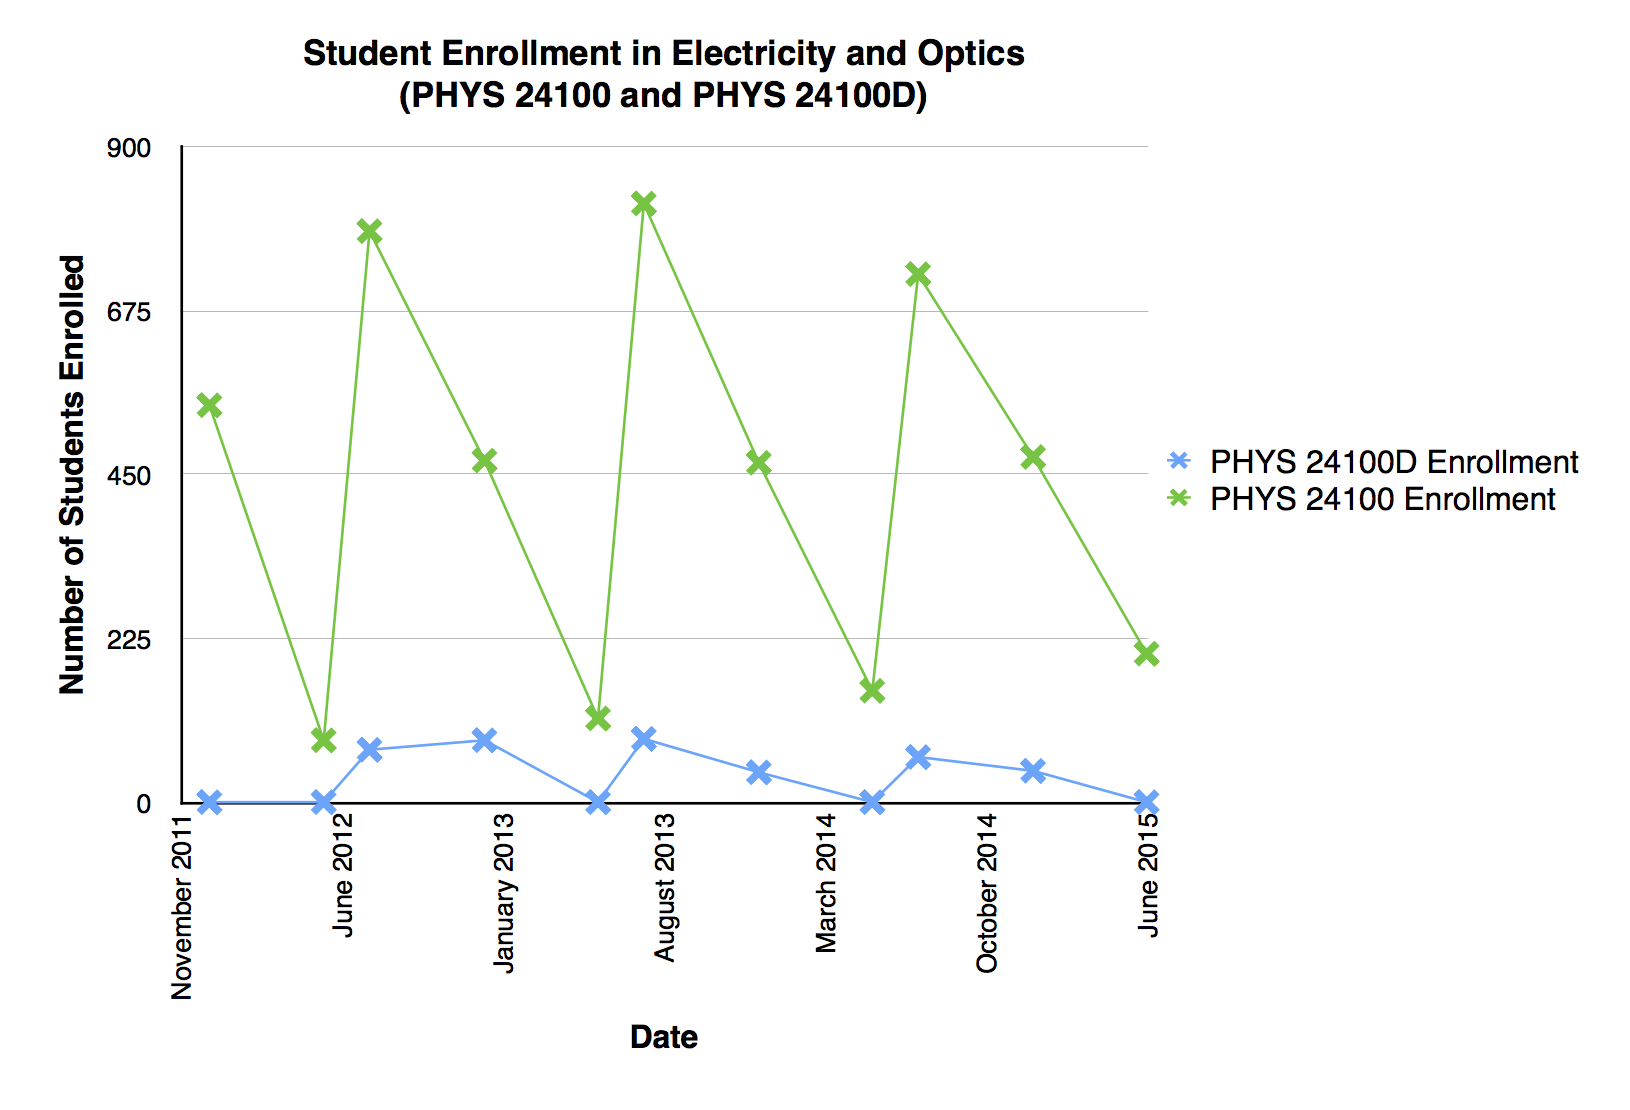
\includegraphics[width=6in]{img/chapter1/enrollment}
	\caption{Enrollment in PHYS 24100 and PHYS 24100D between 2012 and 2015}
	\label{fig:enrollment}
\end{figure}

\begin{figure}
	\centering
	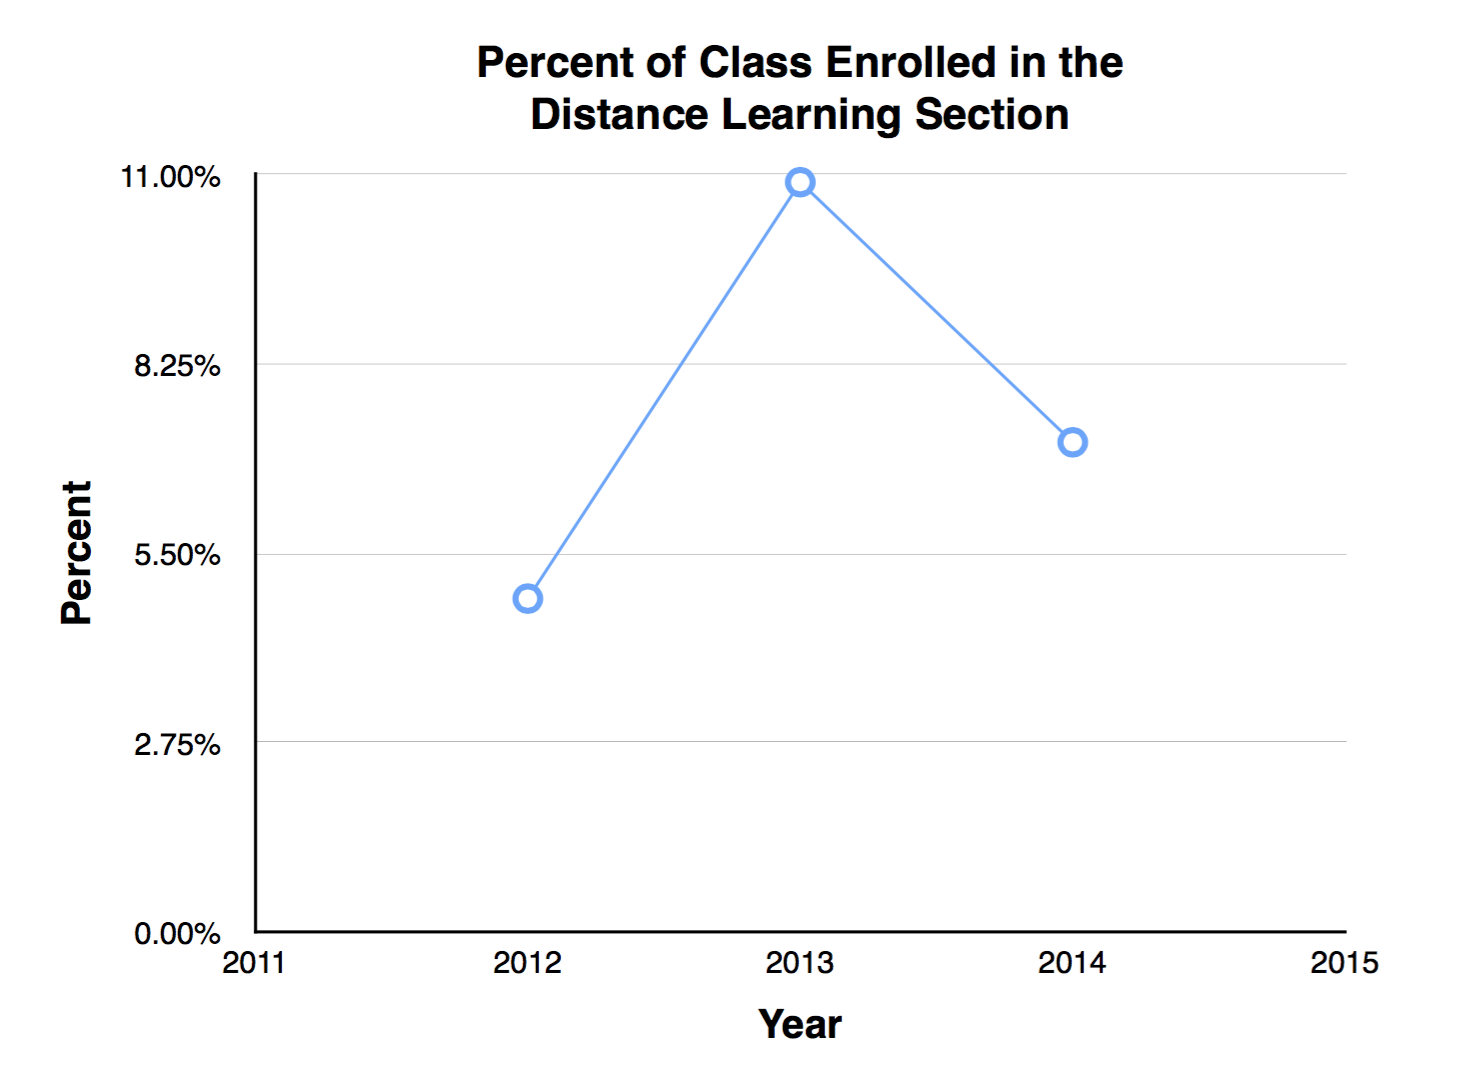
\includegraphics[width=6in]{img/chapter1/percent}
	\caption[Percent of Students Enrolled in PHYS 24100D between 2012 and 2014]{Percent of Students Enrolled in PHYS 24100D between 2012 and 2014}
	\label{fig:percent}
\end{figure}